\documentclass{beamer}

\useoutertheme[subsection=false]{miniframes}
\usecolortheme{beaver}
\setbeamertemplate{navigation symbols}{}
\setbeamertemplate{footline}{}
\usepackage{graphicx}
\usepackage{url}
\usepackage{datetime}
\usepackage{tikz-cd}
\newcommand{\lectureDate}{\formatdate{27}{11}{2018}}

\setbeamertemplate{caption}
{\raggedright\insertcaption\par}
\title{MATH211: Linear Methods I}
\author{Matthew Burke}
\date{\lectureDate}
\begin{document}

\frame{\titlepage}

\begin{frame}{Lecture on \lectureDate}
  \tableofcontents
\end{frame}

\section*{Last time}
\label{sec:Last-time}

\begin{frame}{Last time}
	\begin{itemize}
		\item Multiplication using polar form.\vfill
		\item Complex roots\vfill
		\item Quadratic formula
	\end{itemize}
\end{frame}

\section{Quadratic formula}

\begin{frame}
\begin{beamercolorbox}[sep=12pt,center]{part title}
\usebeamerfont{section title}
\insertsection\par
\end{beamercolorbox}
\end{frame}

\begin{frame}{Examples}
\begin{example}
Solve $z^2-14z+58 = 0$.
\end{example}
\begin{example}
Find a real quadratic with $5-2i$ as a root. What is the other root?
\end{example}
\begin{example}
Solve $z^2-(3-2i)z + (5-i) = 0$.
\end{example}
\end{frame}

\section{Spectral theory}

\begin{frame}
\begin{beamercolorbox}[sep=12pt,center]{part title}
\usebeamerfont{section title}
\insertsection\par
\end{beamercolorbox}
\end{frame}

\begin{frame}{Simplifying matrix actions}
	If
	\begin{equation*}
		A = \left[\begin{matrix}
			3 & -1\\
			-1 & 3
		\end{matrix}\right]
	\end{equation*}
	then $A$ acts on some vectors in a simplified way:
	\begin{equation*}
		A v_1 = 
		A \left[
		\begin{matrix}
		1\\
		1
		\end{matrix}
		\right] = \left[
		\begin{matrix}
		2\\
		2
		\end{matrix}
		\right] = 2v_1
	\end{equation*}
	and
	\begin{equation*}
	\begin{matrix}
	Av_2 =
	A \left[
	\begin{matrix}
	1\\
	-1
	\end{matrix}
	\right] = 
	\left[
	\begin{matrix}
	4\\
	-4
	\end{matrix}
	\right]
	4v_2
	\end{matrix}
	\end{equation*}
\end{frame}

\begin{frame}{Picture}
\begin{columns}
	\column{0.5\textwidth}
	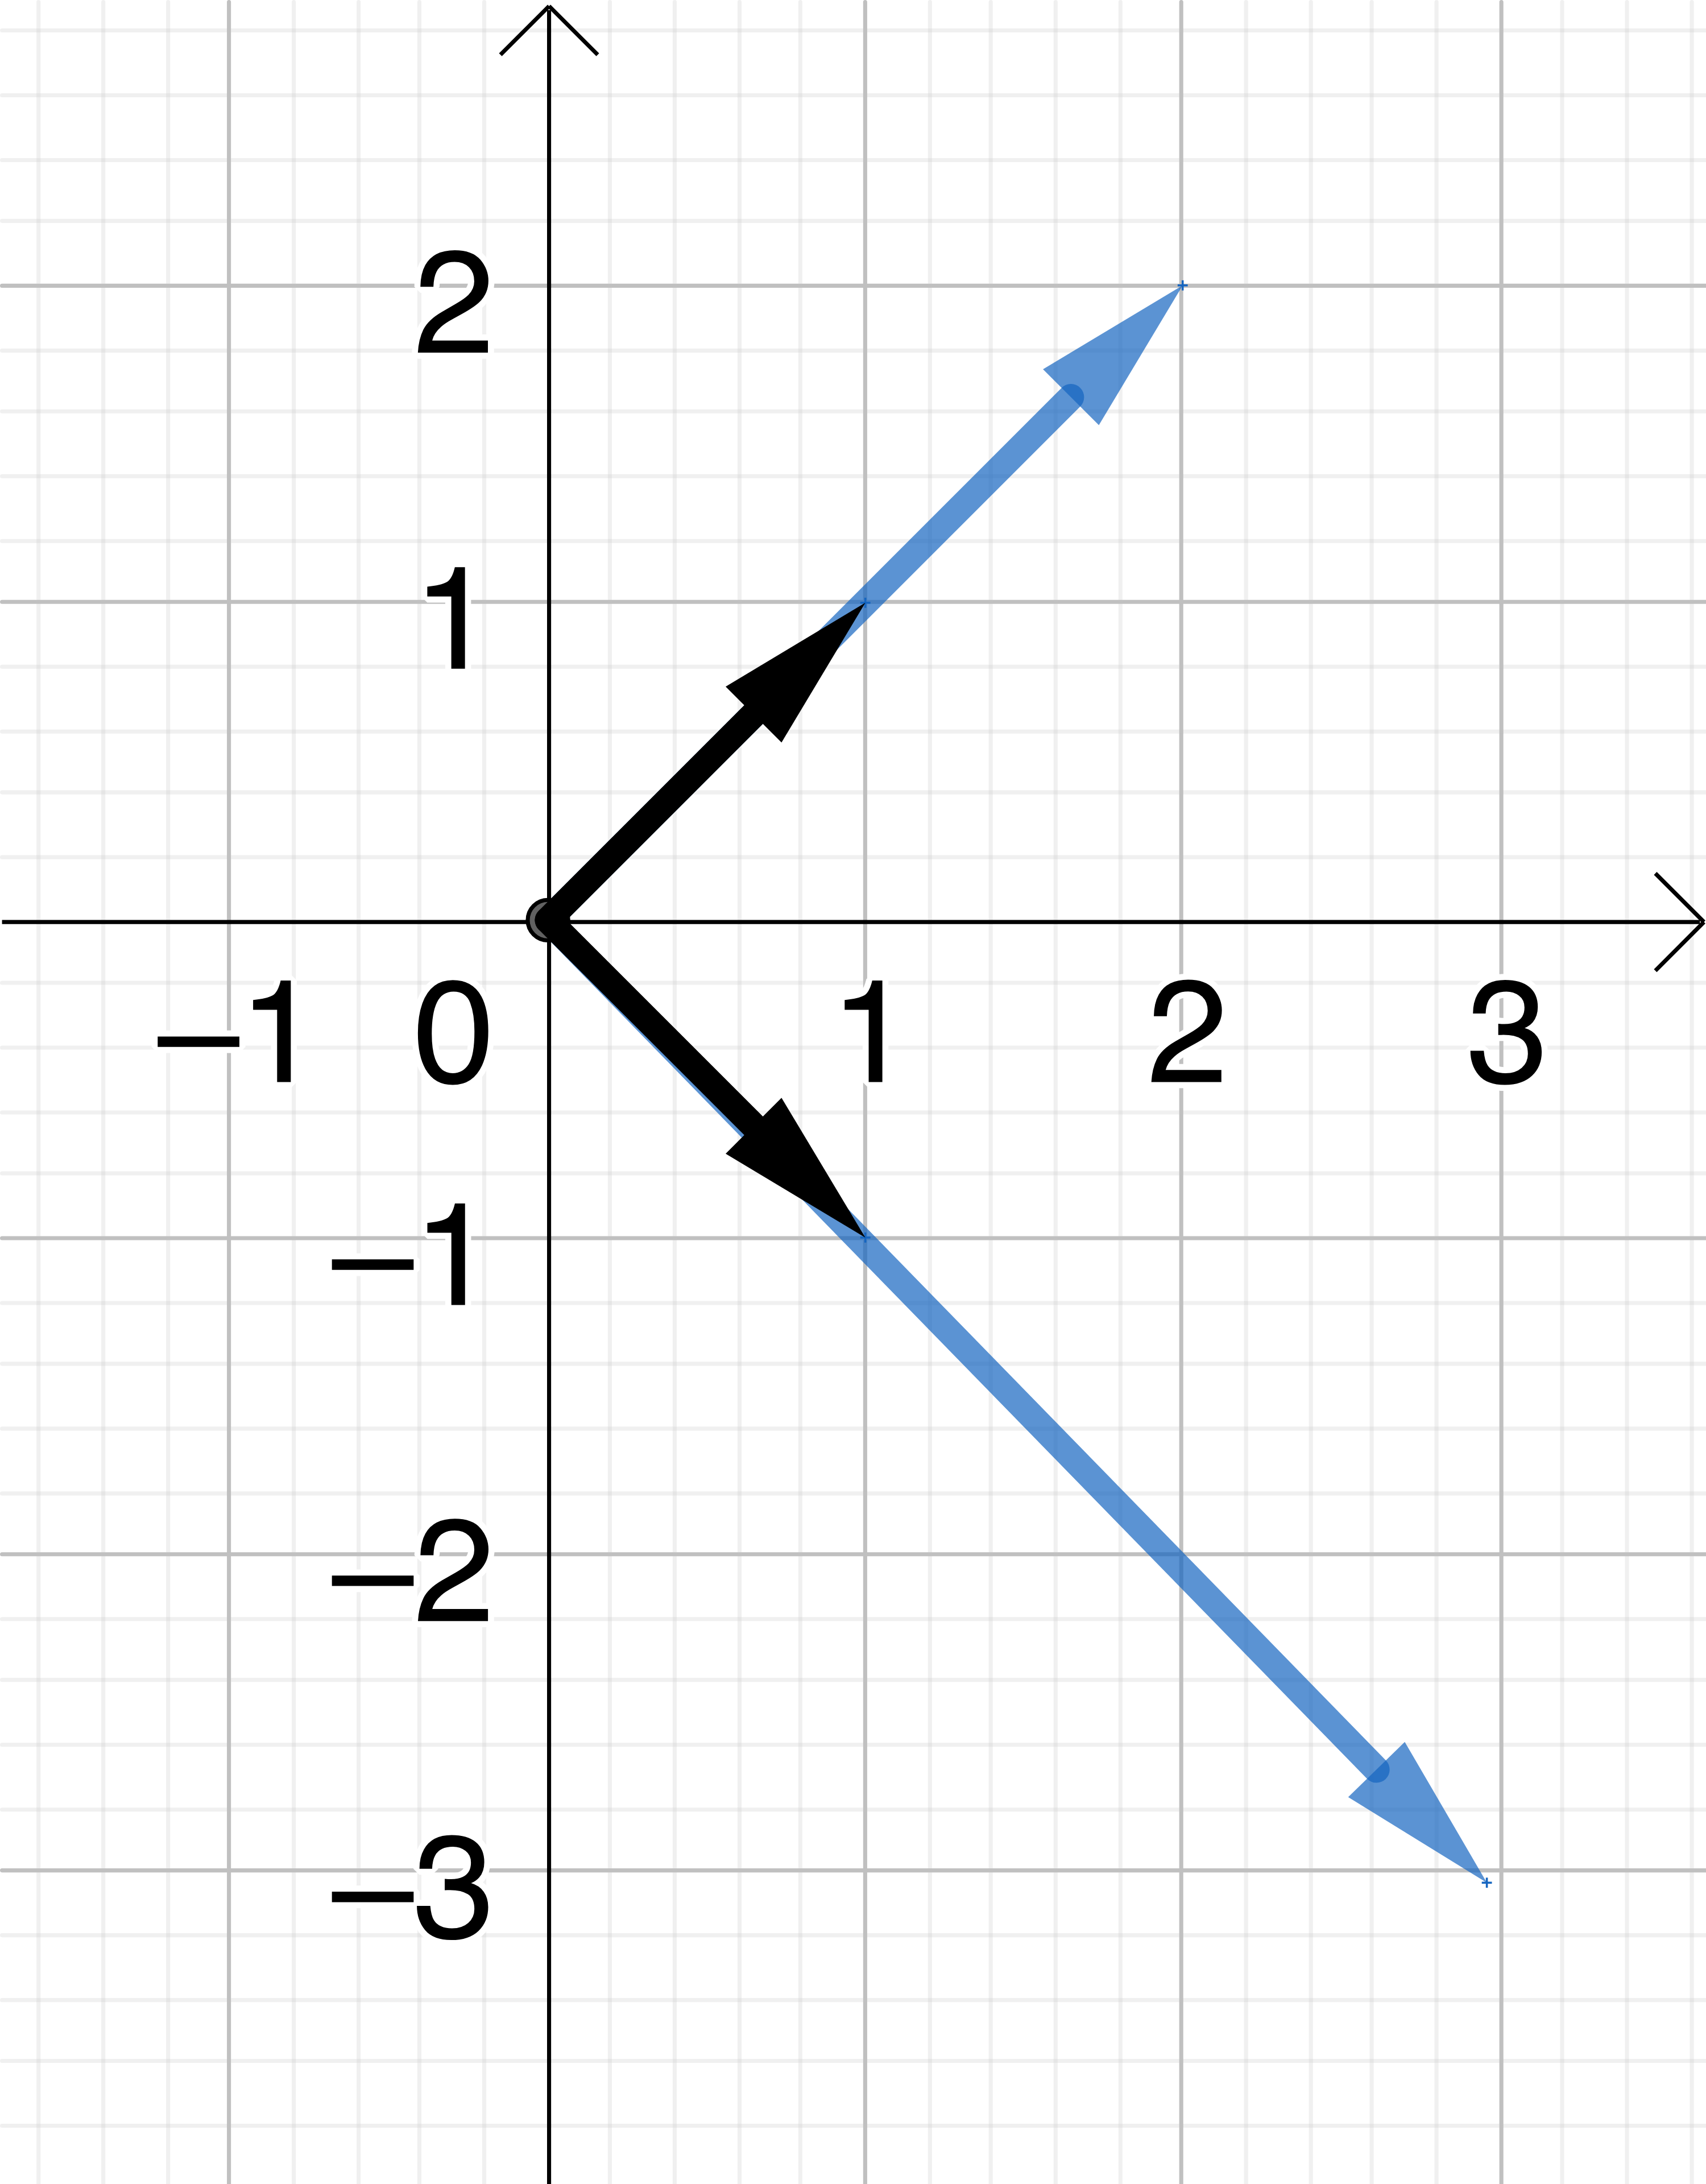
\includegraphics{2d-diag.png}
	\column{0.4\textwidth}
	Since
	\begin{equation*}
		Av_1 = 2v_1
	\end{equation*}
	and
	\begin{equation*}
		Av_2 = 4v_2
	\end{equation*}
\end{columns}
\end{frame}

\begin{frame}{Simplifying matrix actions}
	If
	\begin{equation*}
	A = \frac{1}{2}\left[
	\begin{matrix}
	1&1&2\\
	1&1&-1\\
	-1&1&0
	\end{matrix}
	\right]
	\end{equation*}
	then
	\begin{equation*}
		Av_1 = 
		A \left[
		\begin{matrix}
		1\\
		1\\
		0
		\end{matrix}
		\right] = 
		\left[
		\begin{matrix}
		1\\
		1\\
		0
		\end{matrix}
		\right] = v_1
	\end{equation*}
	\begin{equation*}
		Av_2 =
		A \left[
		\begin{matrix}
		-1\\
		1\\
		0
		\end{matrix}
		\right] = \left[
		\begin{matrix}
		0\\
		0\\
		1
		\end{matrix}
		\right] = v_3
	\end{equation*}
	and
	\begin{equation*}
		Av_3 =
		A \left[
		\begin{matrix}
		0\\
		0\\
		1
		\end{matrix}
		\right] =
		\left[
		\begin{matrix}
		1\\
		-1\\
		0
		\end{matrix}
		\right] = -v_2
	\end{equation*}
\end{frame}

\begin{frame}{Picture}
\begin{columns}
	\column{0.7\textwidth}
	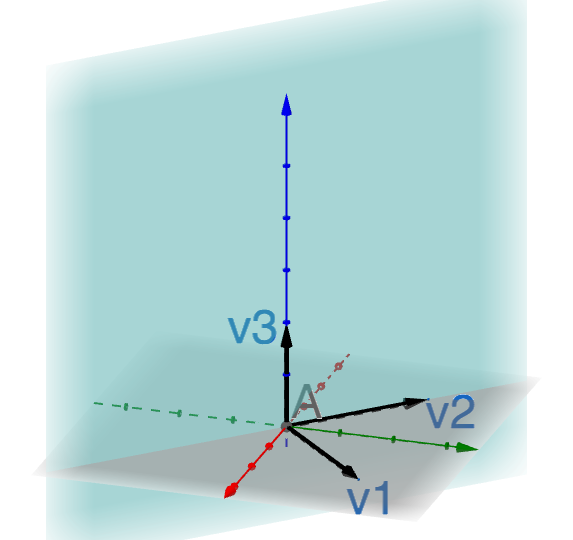
\includegraphics[scale=0.4]{3d-rotation.png}
	\column{0.3\textwidth}
	Blue plane is preserved.
\end{columns}
\end{frame}

\begin{frame}{Eigenvectors and eigenvalues}
\begin{definition}
If $A$ is a square matrix, $v$ is a non-zero vector and
\begin{equation*}
	Av = \lambda v
\end{equation*}
then $A$ has an \emph{eigenvector $v$ with eigenvalue $\lambda$}.
\end{definition}\vfill
{\bf Idea:} If vector $x$ is a linear combination of eigenvectors of $A$ then the action of $A$ on $x$ is easy:
\begin{equation*}
	A(x) = A\left(a_1v_{\lambda_1}+a_2v_{\lambda_2}\right) = a_1A(v_{\lambda_1})+a_2A(v_{\lambda_2}) = a_1\lambda_1v_{\lambda_1}+a_2\lambda_2v_{\lambda_2}
\end{equation*}
\end{frame}

\begin{frame}{Examples}
\begin{example}
$\left[
\begin{matrix}
3&0\\
0&5
\end{matrix}
\right]$ has eigenvectors $\left[
\begin{matrix}
1\\
0
\end{matrix}
\right]$ and $\left[
\begin{matrix}
0\\
1
\end{matrix}
\right]$ with eigenvalues $3$ and $5$ respectively.
\end{example}
\begin{example}
$\left[
\begin{matrix}
3&-1\\
-1&3
\end{matrix}
\right]$ has eigenvectors $\left[
\begin{matrix}
1\\
1
\end{matrix}
\right]$ and $\left[
\begin{matrix}
1\\
-1
\end{matrix}
\right]$ with eigenvalues $2$ and $4$ respectively.
\end{example}
\end{frame}

\section{Eigenvalues}

\begin{frame}
\begin{beamercolorbox}[sep=12pt,center]{part title}
\usebeamerfont{section title}
\insertsection\par
\end{beamercolorbox}
\end{frame}

\begin{frame}{Finding eigenvalues}
Since
\begin{equation*}
Av = \lambda v \iff (A-\lambda I)v = 0
\end{equation*}
and $v\neq 0$ we need to find all $\lambda$ such that 
\begin{equation*}
	A-\lambda I
\end{equation*}
is \emph{not} invertible.
\end{frame}

\begin{frame}{Finding eigenvalues}
\begin{definition}[Characteristic polynomial]
	The \emph{characteristic polynomial of a matrix $A$} is
	\begin{equation*}
	 	\chi_A(\lambda) = det(A-\lambda I)
	 \end{equation*} 
\end{definition}
\begin{itemize}
	\item The eigenvalues are the roots of the characteristic polynomial.
	\item The number of times a root is repeated is called the \emph{algebraic multiplicity} of the root.
	E.g. if
	\begin{equation*}
		\chi_A(\lambda) = (\lambda-4)^3(\lambda+3)(\lambda-1)^2
	\end{equation*}
	then $4$ has algebraic multiplicity $3$, $-3$ has algebraic multiplicity $1$ and $1$ has algebraic multiplicity $2$.
\end{itemize}
\end{frame}

\begin{frame}{Examples}
\begin{example}
	Find the eigenvalues of
	\begin{equation*}
		\left[
		\begin{matrix}
		4&-2\\
		-1&3
		\end{matrix}
		\right]
	\end{equation*}
\end{example}
\begin{example}
	Find the eigenvalues of
	\begin{equation*}
		\left[
		\begin{matrix}
		4&1&2\\
		0&3&-2\\
		0&-1&2
		\end{matrix}
		\right]
	\end{equation*}
\end{example}
\end{frame}

\section{Eigenvectors}

\begin{frame}
\begin{beamercolorbox}[sep=12pt,center]{part title}
\usebeamerfont{section title}
\insertsection\par
\end{beamercolorbox}
\end{frame}

\begin{frame}{Finding eigenvectors}
Suppose that we know $\lambda$ is an eigenvalue for $A$.\vfill
Then we find the eigenvectors associated to $\lambda$ by solving:
\begin{equation*}
(A-\lambda\cdot I)x = 0
\end{equation*}\vfill
\begin{itemize}
	\item After doing row reduction we will get infinitely many solutions.
	\item The no. of parameters is called the \emph{geometric multiplicity} of $\lambda$.
\end{itemize}
\end{frame}

\begin{frame}{Examples}
\begin{example}
	Find the eigenvectors of
	\begin{equation*}
		\left[
		\begin{matrix}
		4&-2\\
		-1&3
		\end{matrix}
		\right]
	\end{equation*}
\end{example}
\begin{example}
	Find the eigenvectors of
	\begin{equation*}
		\left[
		\begin{matrix}
		4&1&2\\
		0&3&-2\\
		0&-1&2
		\end{matrix}
		\right]
	\end{equation*}
\end{example}
\end{frame}


\section{Diagonalisation}

\begin{frame}
\begin{beamercolorbox}[sep=12pt,center]{part title}
\usebeamerfont{section title}
\insertsection\par
\end{beamercolorbox}
\end{frame}

\begin{frame}{Motivation}
If $x\in \mathbb{R}^n$ is a linear combination of eigenvectors of $A$ then:
\begin{equation*}
	A(x) = A\left(\sum_{i=1}^n a_i v_{\lambda_i}\right) = \sum_{i=1}^n a_iA(v_{\lambda_i}) = \sum_{i=1}^n a_i\lambda_iv_{\lambda_i}
\end{equation*}
So if \emph{every} vector in $\mathbb{R}^n$ can be written as a linear combination of eigenvectors of $A$ the the \emph{entire} matrix action simplifies.\vfill
\begin{definition}
	An $n\times n$ matrix $A$ is \emph{diagonalisable} iff every vector in $\mathbb{R}^n$ can be written as a linear combination of eigenvectors.
\end{definition}
\end{frame}

\begin{frame}{Motivation}
Suppose we want to find 
\end{frame}


\end{document}